\section{Results}

In this section we present a collection of simple experiments to demonstrate various features of the
proposed algorithm.


\subsection{Smoothing Comparison}
\label{sec:LeafSmoothingComparison}

In Section \S\ref{sec:modelingFluenceBlocking} we describe a smooth model of how the leaves block radiation.
Here we describe do a simple experiment to look at how adjusting that smoothing parameter affects the optimization.

We uses a single target fluence profile, as shown in Figure \ref{fig:fluenceMapSmoothingExample},
and assumes that the dose-rate is a constant function of time.
We performed a simple grid search, computing the optimal leaf trajectories for each dose-rate value.
We then ran this grid-search twice, once with heavy smoothing and once with light smoothing.

The smoothing parameter can be expressed in terms of a characteristic blurring width.
Here we used a width of 0.5 cm for the heavy smoothing and 0.05 cm for the light smoothing.
The characteristic width was computed such that the smoothing function achieved 95\% of its
change in value over the smoothing window.

We also used seven of leaf trajectory segments, although similar results are obtained for trajectories with more segments.
\todo{add a figure for that? Or maybe another sub-section?}
This number was computed with a pilot study.
Fewer trajectory segments lead to faster solve times, but the fitting error increases significantly.
Using more trajectory segments takes longer, but at a trivial reduction in fitting error.

Figure \ref{fig:smoothVsStiffOptimization} shows the two sequences of optimizations, one for the
heavy smoothing of 0.5 cm and the other for the light smoothing of 0.05 cm.
The objective function is normalized by the fitting error associated with a solution where the
leaves completely block the radiation.
Although both optimizations are able to find reasonable solutions, there are a few salient differences.
The optimization with light smoothing takes about four times longer to run when
compared to the optimization with heavy smoothing.
The optimization with light smoothing also tends to get stuck in local minima, as shown by the
objective function jumping around with small changes in the constant dose-rate.
The optimization with heavy smoothing eventually converges to trajectories that rely on the
smoothing behavior to achieve the desired fluence profile. This is clear from the discrepancy
between the smooth and exact model for dose rates above 4 MU.
That being said, this discrepancy between the models is small and the overall shape of the delivered
fluence map is generally correct, as shown in Figure \ref{fig:smoothVsStiffOptimization}.

\begin{figure}
  \centering
  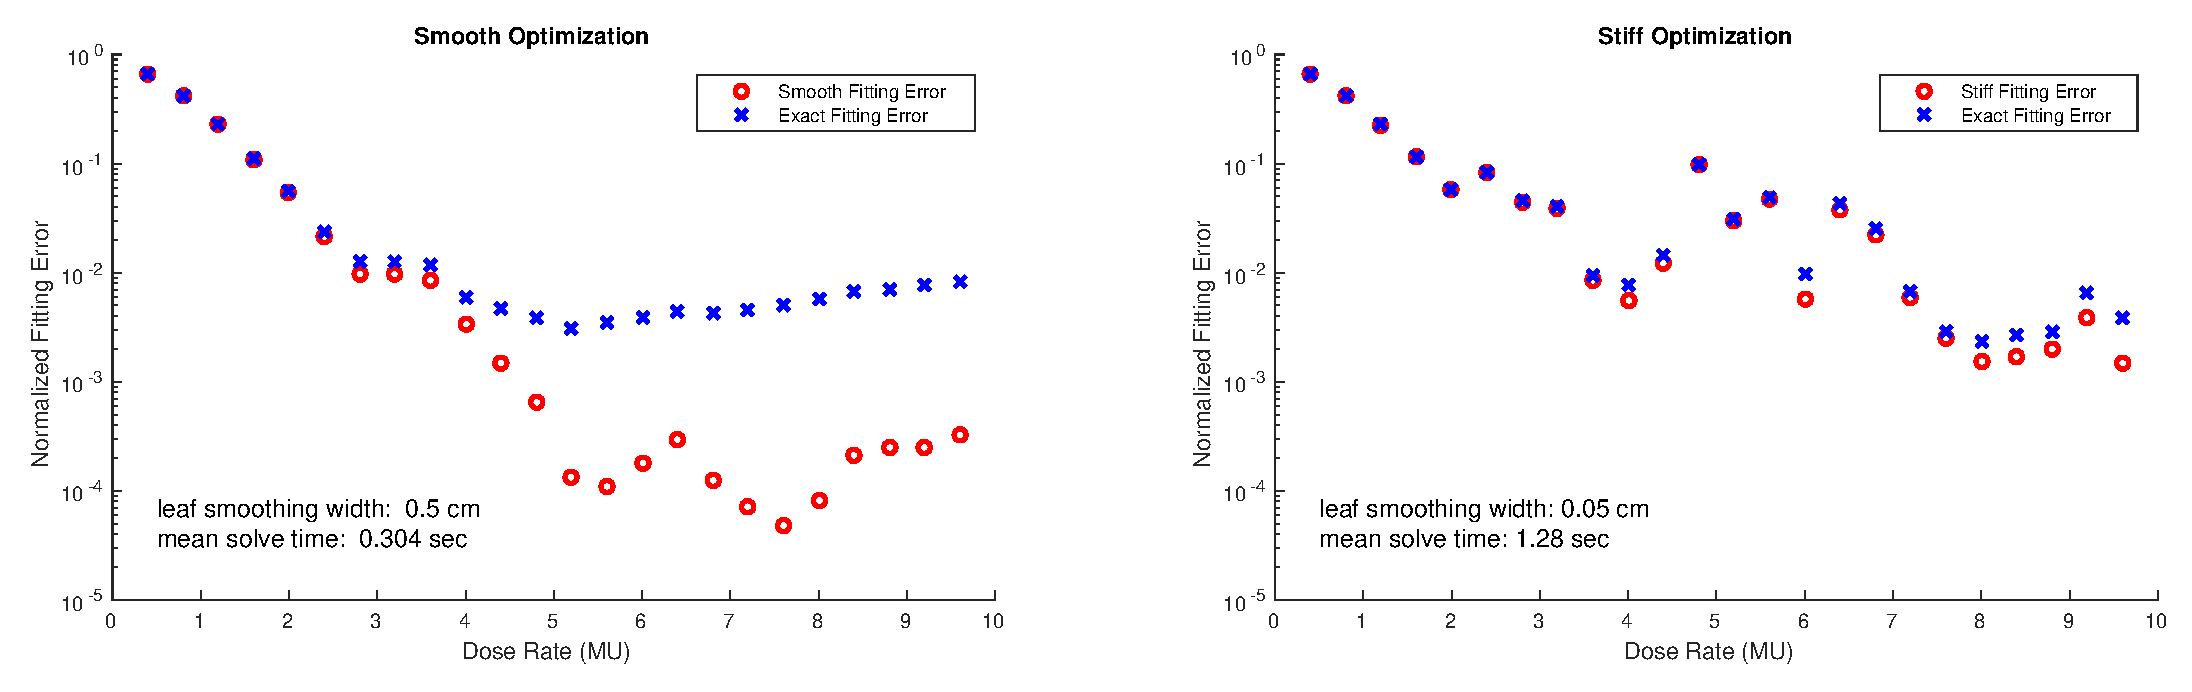
\includegraphics[width=\textwidth]{fig/smoothVsStiffOptimization.pdf}
  \caption{Comparison of heavy and light smoothing in leaf-blocking model.
           In each plot we ran 24 leaf optimizations, sweeping through a range of constant dose-rate trajectories.
           The optimizations in the left plot used a leaf smoothing distance of 0.5 cm, while the
           right plot used 0.05 cm.
           Notice that the left set of optimization does a better job of avoiding local minima,
           but that there is a disparity between the fluence profile produced by the smooth model
           and the exact (no smoothing) model.
           The right plot does better job of matching the exact model, but it tends to get stuck in local minima
           and takes significantly (4x) longer to run.
           The solution for a dose rate of 5.2 MU on the left plot is
           shown in detail in Figure \ref{fig:fluenceMapSmoothingExample}.
          }
  \label{fig:smoothVsStiffOptimization}
\end{figure}

\begin{figure}
  \centering
  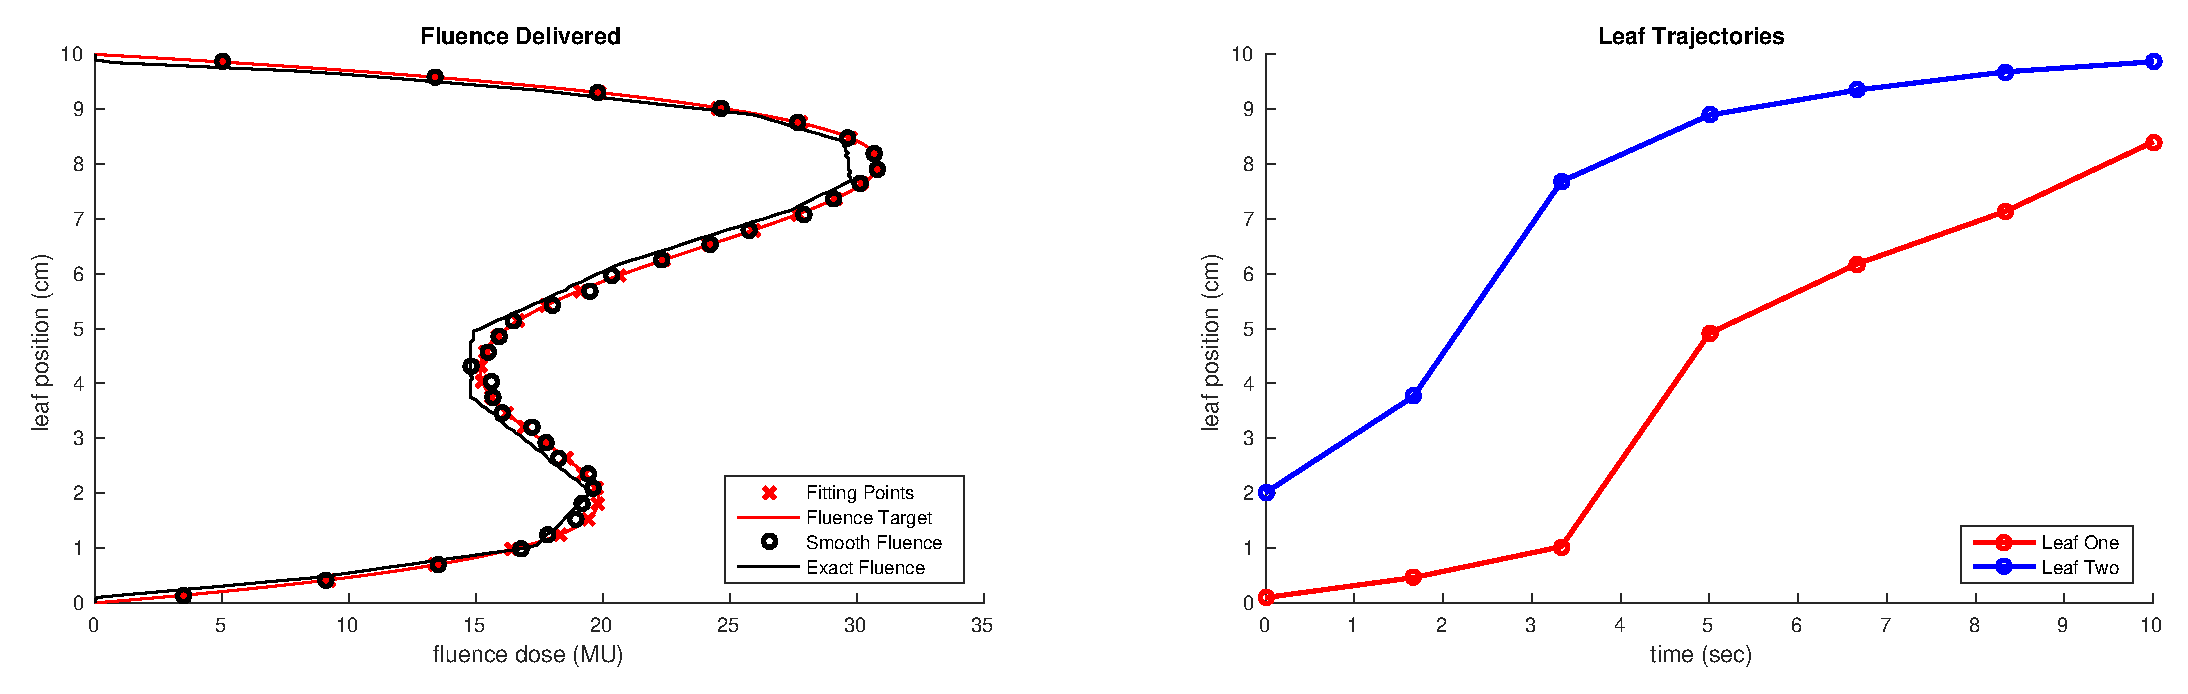
\includegraphics[width=\textwidth]{fig/fluenceMapSmoothingExample.pdf}
  \caption{ Optimal leaf-trajectories, computed with a smoothing width of 0.5 cm and a constant
            dose-rate of 5.2 MU. Note the small discrepancy between the smooth model of the
            delivered fluence and the exact (no smoothing) model.}
  \label{fig:fluenceMapSmoothingExample}
\end{figure}


\subsection{Iterative Smoothing Refinement}

One common trick in trajectory optimization is to solve a trajectory optimization problem
iteratively, making small adjustments to the problem statement between each optimization,
and using the result of the previous optimization to seed the next.

We can do this iterative refinement with the leaf-blocking smoothing parameter,
starting with heavy smoothing and then using that solution to seed another optimization
with a smaller smoothing term.

We test this procedure by doing an experiment similar to the one discussed in
\S Section \ref{sec:LeafSmoothingComparison}, but using the solution of the heavy-smoothing
optimization to initialize the optimization with light smoothing.
Here we will use a sequence of three optimizations, starting with a smoothing of
0.5 cm, then moving to 0.1 cm, and finally 0.05 cm for the final optimization.

The resulting sweep of optimizations is shown in Figure \ref{fig:iterSmoothSweep}.
These results are better than either the heavy or light smoothing optimizations.
The total optimization time for all three optimizations is less than simply running the
light smoothing optimization from a niave guess, the model discrepancy is tiny, and the
solver is generally able to do a good job of avoiding local minima.

\begin{figure}
  \centering
  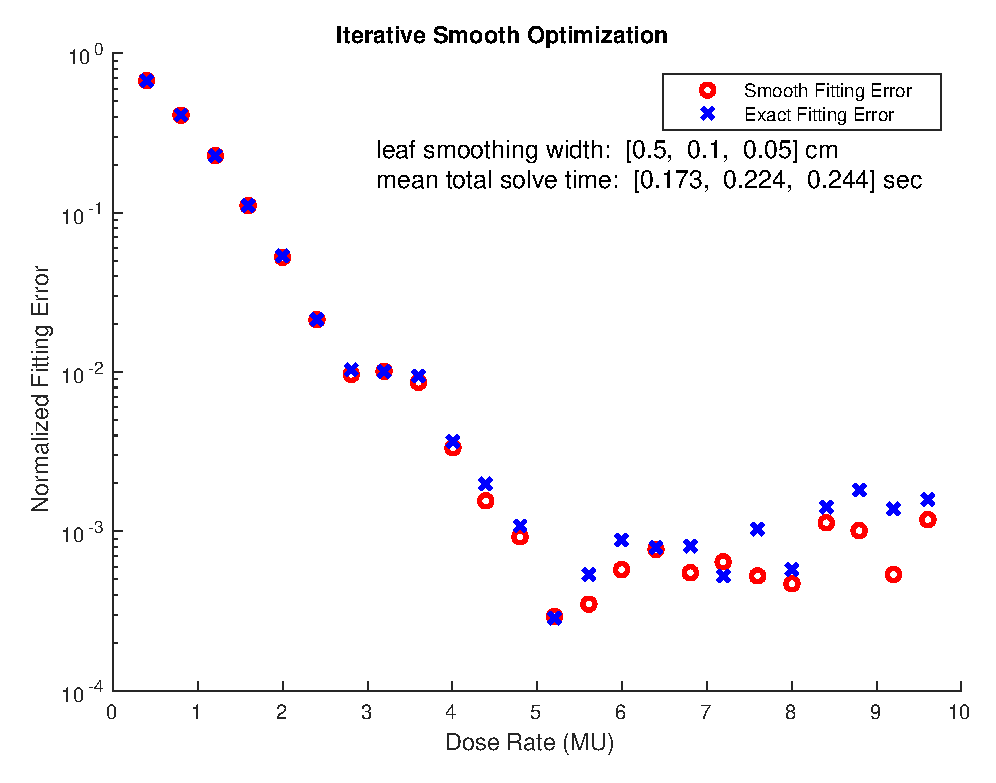
\includegraphics[width=3in]{fig/iterSmoothSweep.pdf}
  \caption{This plot shows the objective function value for the optimal leaf trajectories,
           given a constant fluence dose rate. Each optimization here is actually a set of three
           optimizations, each using a successively smaller smoothing distance. In all cases
           the first optimization used a smoothing distance of 0.5cm, the second used 0.1cm,
           and the final optimization used 0.05cm. This technique results in faster solve times
           than a single optimization with the smallest smoothing parameter, while also avoiding
           local minima.}
  \label{fig:iterSmoothSweep}
\end{figure}

Figure \ref{fig:fluenceMapIterativeBest} again shows the optimal leaf trajectories with a
constant dose rate of 5.2 MU. The leaf trajectories are qualitatively similar to those in
Figure \ref{fig:fluenceMapSmoothingExample}, but slight changes are present that make the
exact-model fluence profile much closer to the target profile.

\begin{figure}
  \centering
  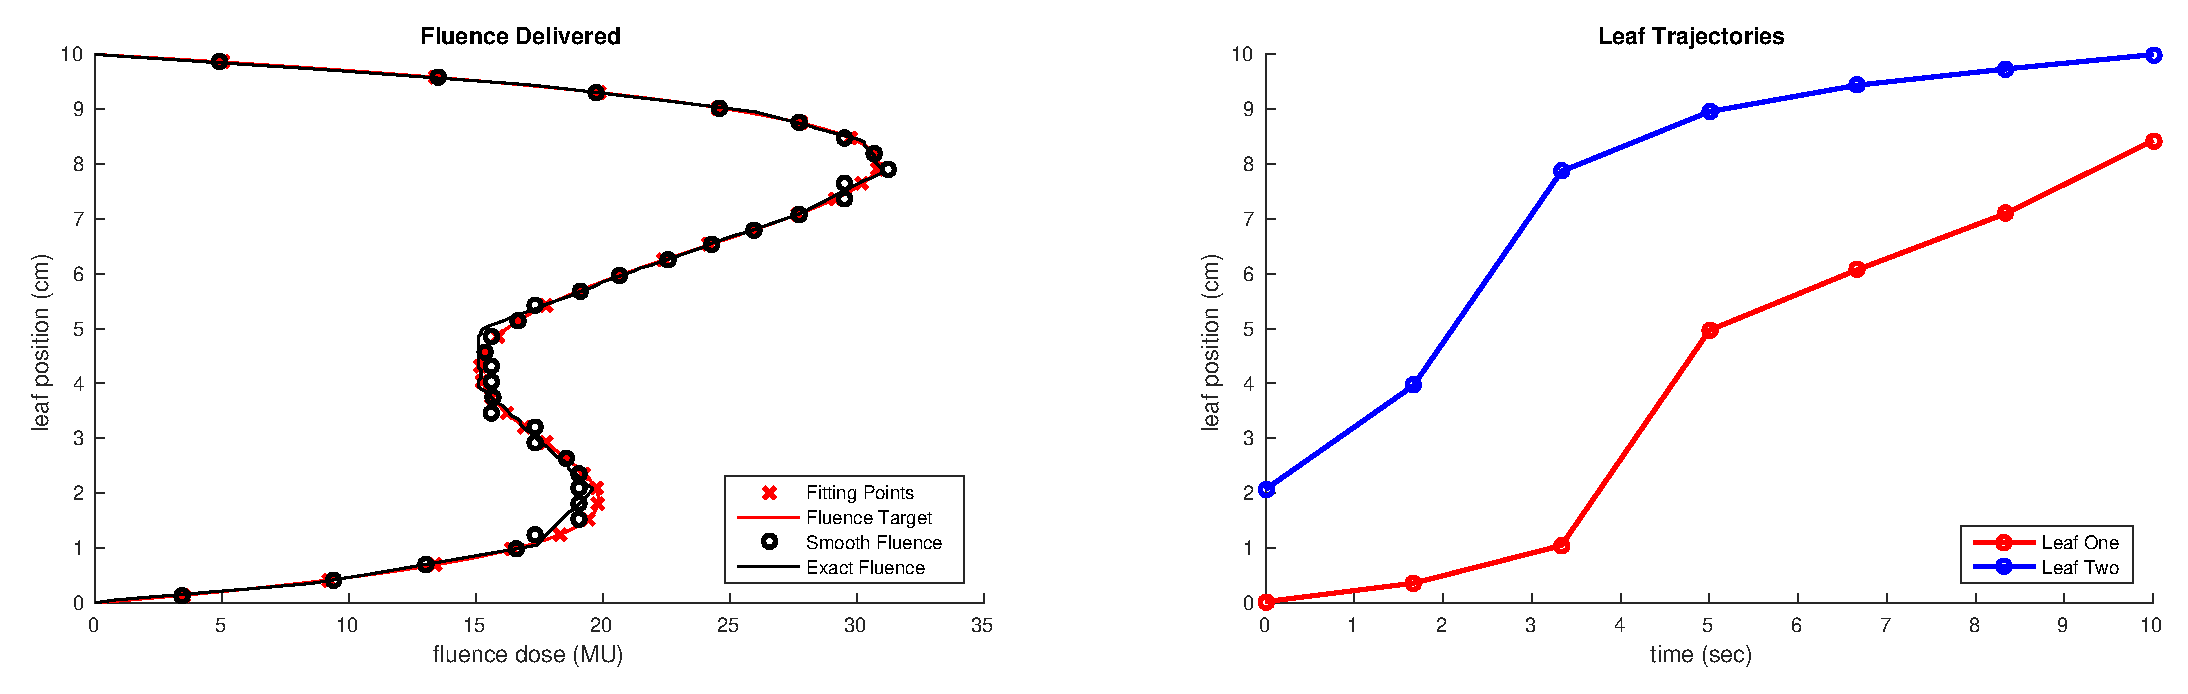
\includegraphics[width=\textwidth]{fig/fluenceMapIterativeBest.pdf}
  \caption{This plot shows the optimal leaf trajectories and delivered fluence map using the
           best solution (dose rate = 5.2 MU) found by the iterative optimization procedure.
           Note that these trajectories are similar to those in
           Figure \ref{fig:fluenceMapSmoothingExample}, but that the fitting is better here.}
  \label{fig:fluenceMapIterativeBest}
\end{figure}


\subsection{Computing Dose-rate Trajectories}

\todo{CMAES optimization for a single trajectory?}

\subsection{Multi-VMAT}

\todo{David - should we try to run an optimization with multiple pairs of leaves?}

\subsection{Misc. Notes:}

\todo{Clean up this section, perhaps add a few small plots.}

It seems that the velocity smoothing has little effect on the optimization: no significant
change observed in computation time, convergence, or trajectories.

The number of fitting points is important -- if there are too few the the trajectories tend to
become less smooth and more local minima pop up. I believe that this is caused by overfitting.

The solve time varies linearly with number of trajectory segments, at least on the range of 7 to 13 segments.
The solution quality does not appear to change that much, although a few extra bumps do appear in the trajectories.
If there are too few points, then the it is sometimes not possible to capture some features in the target profile.
